\documentclass{ximera}
\graphicspath{{./auto_generated_text/Week1CoordinateSystems/graphics/}{./graphics/}}
\title{Practice Problems}
\begin{document}
\begin{abstract}
\end{abstract}
\maketitle
\section{Online Problems}
\begin{problem}
Find the Cartesian coordinates of each point, which is given in polar coordinates.

$(r,\theta) = (2, \pi/6)$
\[
(x,y) = \answer{(\sqrt{3},1)}
\]
$(r,\theta) = (\sqrt{2}, 3\pi/4)$
\[
(x,y) = \answer{(-1,1)}
\]
$(r,\theta) = (1, 0)$
\[
(x,y) = \answer{(1,0)}
\]
$(r,\theta) = (3, \pi)$
\[
(x,y) = \answer{(-3,0)}
\]
\end{problem}

\begin{problem}
Find the polar coordinates of each point, which is given in Cartesian coordinates. Your answers should satify $0\leq r$ and $0\leq \theta < 2\pi$.

$(x,y) = (\sqrt{3},0)$
\[
(r,\theta) = \answer{(\sqrt{3},0)}
\]
$(x,y) = (0,2)$
\[
(r,\theta) = \answer{(2,\pi/2)}
\]
$(x,y) = (-1,-1)$
\[
(r,\theta) = \answer{(\sqrt{2},5\pi/4)}
\]
$(x,y) = (1,\sqrt{3})$
\[
(r,\theta) = \answer{(2,\pi/3)}
\]
\end{problem}

\begin{problem}
Find the Cartesian coordinates of the point $(\pi/2, \pi, 2)$, given in cylindrical coordinates.
\[
(x,y,z) = \answer{(0, -\pi/2, 2)}
\]
\end{problem}

\begin{problem}
Find cylindrical coordinates for the point $\left(0, -1, 3\right)$, written in Cartesian coordinates. Your answer should satisfy $0\leq r$ and $0\leq \theta <2\pi$.
\[
(r, \theta, z) = \answer{(1, \pi, 3)}
\]
\end{problem}

\begin{problem}
Consider the surface described in Cartesian coordinates by
\[
2z^2 = x^2 +y^2.
\]
Describe this surface with an equation in cylindrical coordinates, of the form $0=f(r,\theta, z)$.
\[
0=\answer{r^2-2z^2}
\]
FIGURE OUT HOW TO HANDLE THIS!!!
What type of shape is this?
\begin{multipleChoice}
\choice{Plane}
\choice{Cylinder}
\choice{Sphere}
\choice[correct]{Cone}
\choice{Other}
\end{multipleChoice}
\end{problem}

\begin{problem}
Consider the following region in $\mathbb{R}^3$.

\begin{image}
\begin{tikzpicture}
\node[inner sep=0pt] at (0,0)
    {
\includegraphics{cylinder_wedge}};
\end{tikzpicture}
\end{image}

This region is the set of points $(r, \theta, z)$, in cylindrical coordinates, satisfying the inequalities
\begin{align*}
&\answer{1}\leq r\leq \answer{2}\\
&\answer{\pi/2}\leq\theta\leq\answer{\pi}\\
&\answer{-1}\leq z\leq\answer{1}
\end{align*}

\end{problem}

\begin{problem}
For each of the following equations in cylindrical coordinates, select the type of shape they define.

FIGURE OUT CORRECT ANSWERS

$r = \cos\theta$
\begin{multipleChoice}
\choice{plane}
\choice{cylinder}
\choice{sphere}
\choice{other}
\end{multipleChoice}

$z = r\cos\theta$
\begin{multipleChoice}
\choice{plane}
\choice{cylinder}
\choice{sphere}
\choice{other}
\end{multipleChoice}

$z = -r$
\begin{multipleChoice}
\choice[correct]{plane}
\choice{cylinder}
\choice{sphere}
\choice{other}
\end{multipleChoice}
\end{problem}

\begin{problem}
Find the Cartesian coordinates of each point, given in cylindrical coordinates.

$(r,\theta,z) = (1,1,1)$
\[
(x,y,z) = \answer{(\cos(1), \sin(1), 1)}
\]
$(r,\theta,z) = (\pi,\pi,\pi)$
\[
(x,y,z) = \answer{(-\pi, 0, \pi)}
\]
$(r,\theta,z) = (2,4\pi/3,-2)$
\[
(x,y,z) = \answer{(-\sqrt{3}, -1, -2)}
\]
\end{problem}

\begin{problem}
Find the cylindrical coordinates of each point, given in Cartesian coordinates. Your answers should satisfy $r\geq 0$ and $0\leq \theta < 2\pi$.

$(x,y,z) = (1,1,1)$
\[
(r,\theta,z) = \answer{(\sqrt{2}, \pi/4, 1)}
\]
$(x,y,z) = (\pi,\pi,\pi)$
\[
(r,\theta,z) = \answer{(\sqrt{2}\pi, \pi/4, \pi)}
\]
$(x,y,z) = (2,2\sqrt{3},-2)$
\[
(r,\theta,z) = \answer{(4, \pi/6, -2)}
\]
\end{problem}

\begin{problem}
Find the Cartesian coordinates of the point $(2, \pi, \pi/2)$, given in spherical coordinates.
\[
(x,y,z) = \answer{(-2,0,0)}
\]
\end{problem}

\begin{problem}
Find spherical coordinates for the point $\left(-\sqrt{2}, \sqrt{2}, 2\sqrt{3}\right)$, written in Cartesian coordinates. Your answer should satisfy $0\leq \rho$, $0\leq \theta \leq 2\pi$, and $0\leq \phi \leq \phi$.
\[
(\rho, \theta, \phi) = \answer{(4, 3\pi/4, \pi/6)}
\]
\end{problem}

\begin{problem}
Consider the surface described in Cartesian coordinates by
\[
2z^2 = x^2 +y^2.
\]
Describe this surface with an equation in spherical coordinates, of the form $0=f(\rho, \theta, \phi)$.
\[
0=\answer{\rho^2\sin^2\phi - 2\cos^2\phi}
\]
FIGURE OUT HOW TO HANDLE THIS!!!
What type of shape is this?
\begin{multipleChoice}
\choice{Plane}
\choice{Cylinder}
\choice{Sphere}
\choice[correct]{Cone}
\choice{Other}
\end{multipleChoice}
\end{problem}

\begin{problem}
Consider the following region in $\mathbb{R}^3$.

\begin{image}
\begin{tikzpicture}
\node[inner sep=0pt] at (0,0)
    {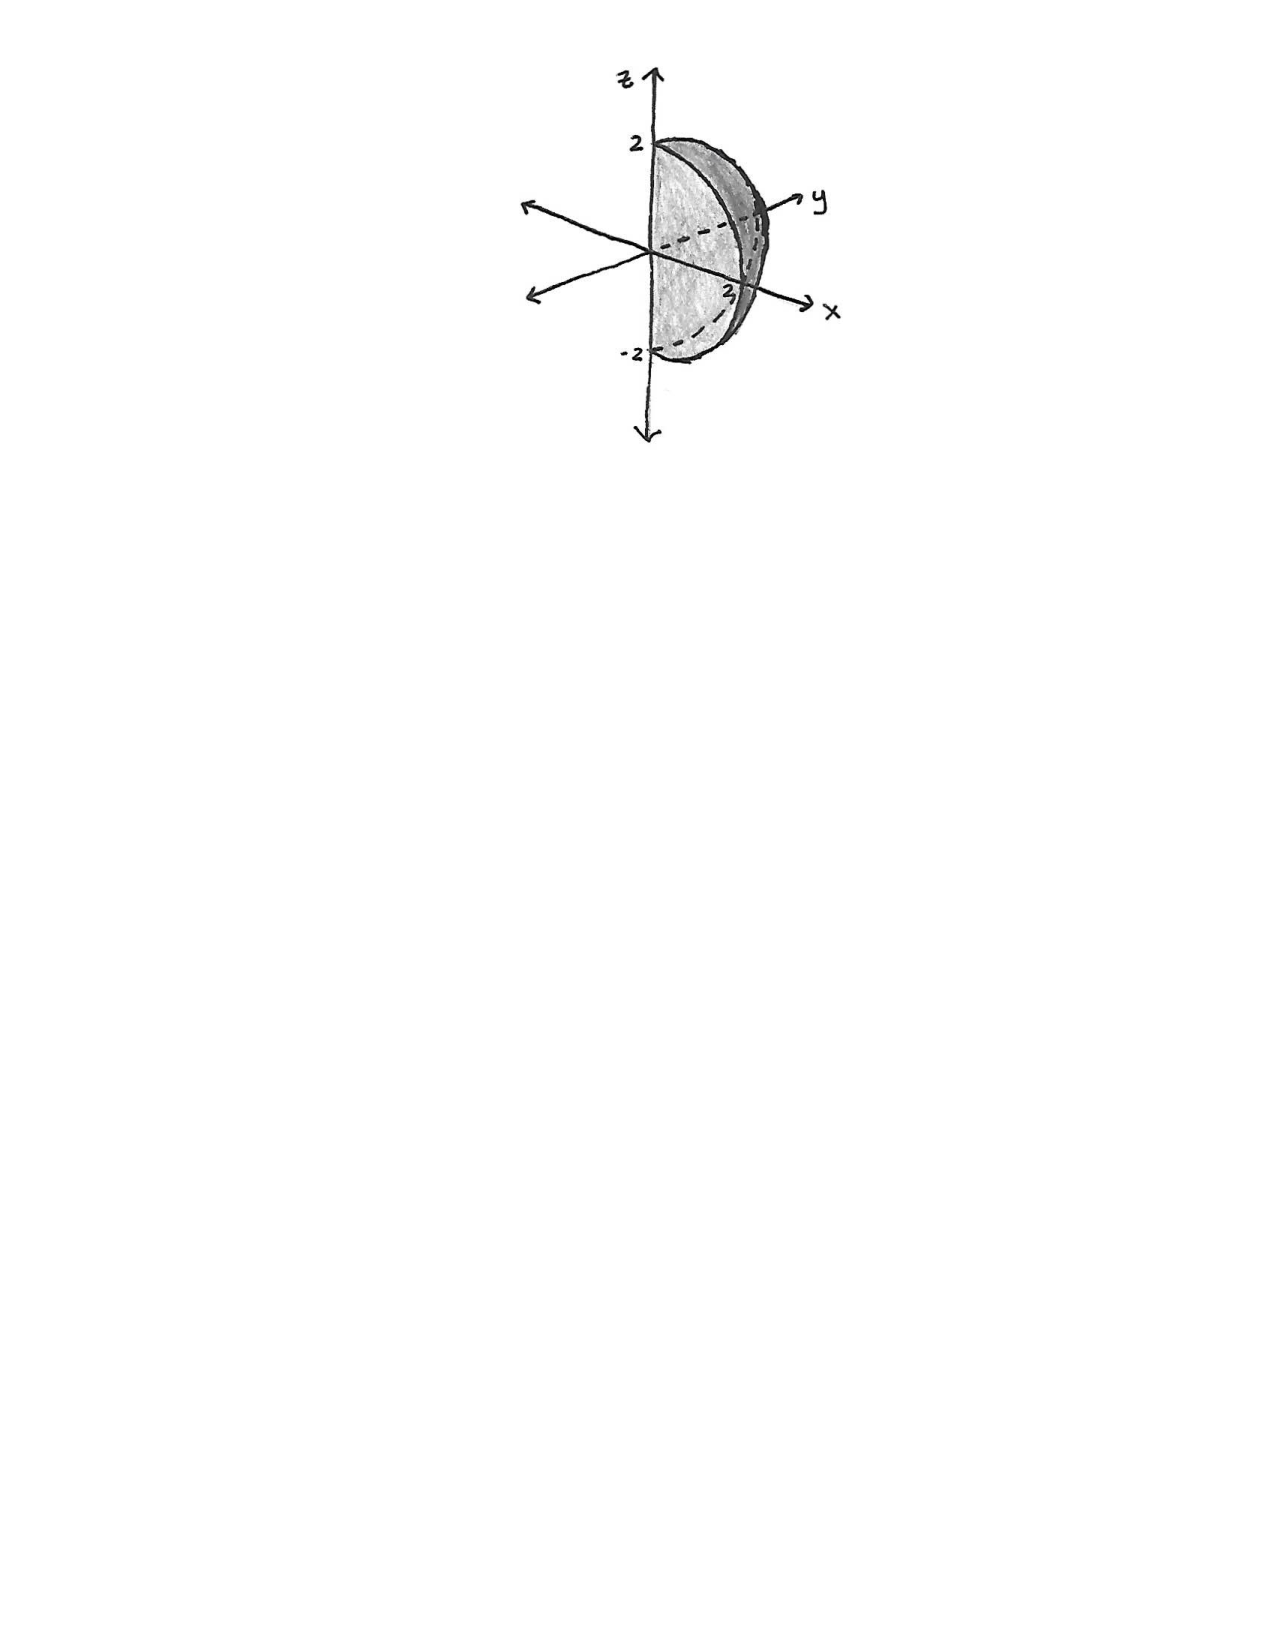
\includegraphics{sphere_wedge}};
\end{tikzpicture}
\end{image}

This region is the set of points $(\rho,\theta,\phi)$, in spherical coordinates, satisfying the inequalities
\begin{align*}
&\answer{0}\leq\rho\leq \answer{2}\\
&\answer{0}\leq\theta\leq\answer{pi/2}\\
&\answer{0}\leq\phi\leq\answer{pi}
\end{align*}

\end{problem}

\begin{problem}
For each of the following equations in spherical coordinates, select the type of shape they define.

FIGURE OUT CORRECT ANSWERS

$\rho = \cos\phi$
\begin{multipleChoice}
\choice{plane}
\choice{cylinder}
\choice{sphere}
\choice{other}
\end{multipleChoice}

$\rho = \sin\theta$
\begin{multipleChoice}
\choice{plane}
\choice{cylinder}
\choice{sphere}
\choice{other}
\end{multipleChoice}

$\rho\cos\theta\sin\phi = 1$
\begin{multipleChoice}
\choice[correct]{plane}
\choice{cylinder}
\choice{sphere}
\choice{other}
\end{multipleChoice}
\end{problem}

\begin{problem}
Find the spherical coordinates of each point, given in Cartesian coordinates. Your answers should satisfy $0\leq r$, $0\leq\theta < 2\pi$, and $0\leq \phi\leq \pi$.

$(x,y,z) = (1,1,1)$
\[
(\rho,\theta,\phi) = \answer{(\sqrt{3}, \pi/4, \pi/4)}
\]
$(x,y,z) = (1, -1, -1)$
\[
(\rho,\theta,\phi) = \answer{(\sqrt{3}, 3\pi/4, 3\pi/4)}
\]
$(x,y,z) = (1,\sqrt{3},0)$
\[
(\rho,\theta,\phi) = \answer{(\sqrt{4}, \pi/6, \pi/2)}
\]
\end{problem}

\begin{problem}
Find the Cartesian coordinates of each point, given in spherical coordinates.

$(\rho,\theta,\phi) = (\pi,\pi,\pi)$
\[
(x,y,z) = \answer{(0, 0, -\pi)}
\]
$(\rho,\theta,\phi) = (3,\pi/2,\pi/4)$
\[
(x,y,z) = \answer{(0, 3\sqrt{2}/2, 3\sqrt{2}/2)}
\]
$(\rho,\theta,\phi) = (2,7\pi/6,3\pi/4)$
\[
(x,y,z) = \answer{(-\sqrt{6}/2, -\sqrt{2}/2, -\sqrt{2})}
\]

\end{problem}


\section{Written Problems}
\begin{problem}
For several values of the constant $a$, sketch the graph of the curve in $\mathbb{R}^2$ given by the polar equation
\[
r = a\sin\theta .
\]
What do you notice about these curves?
\end{problem}

\begin{problem}
Which points in $\mathbb{R}^2$ have the same coordinates when written in Cartesian and polar coordinates? (That is, for what points do we have $x=r$ and $y=\theta$?)
\end{problem}

\begin{problem}
Consider the surface described by $(r-3)^2 +z^2 = 1$ in cylindrical coordinates, with the restriction $r\geq 0$.
\begin{enumerate}
\item Sketch the intersection of the surface with the half-plane $\theta = 0$.
\item Sketch the intersection of the surface with the half-plane $\theta = \frac{\pi}{2}$.
\item Sketch the intersection of the surface with the plane $z = 0$. 
\item Sketch the surface.
\end{enumerate}
\end{problem}

\begin{problem}
Sketch the region in $\mathbb{R}^3$ with cylindrical coordinates satisfying the inequality
\[
r\leq z \leq 4-2r
\]
\end{problem}

\begin{problem}
Convert the following equation, given in cylindrical coordinates, into Cartesian coordinates.
\[
r = 0
\]
\end{problem}

\begin{problem}
Sketch the region in $\mathbb{R}^3$ given by
\begin{align*}
&r\leq z\leq 3\\
&0\leq\theta \leq\pi/2
\end{align*}
in cylindrical coordinates.
\end{problem}

\begin{problem}
Sketch the region in $\mathbb{R}^3$ given by
\[
r^2-2\leq z\leq 2-r^2
\]
in cylindrical coordinates.

\end{problem}

\begin{problem}
Which points in $\mathbb{R}^3$ have the same coordinates when written in Cartesian and cylindrical coordinates?
\end{problem}

\begin{problem}
\begin{enumerate}
\item Given a function $f$, consider the graphs of the equations $r = f(\theta)$ and $r = 2f(\theta)$, in polar coordinates. How are these graphs related?
\item Given a function $f$, consider the graphs of the equations $\rho = f(\theta, \phi)$ and $\rho = 2f(\theta, \phi)$, in spherical coordinates. How are these graphs related?
\item Given a function $f$, consider the graphs of the equations $r = f(\theta)$ and $r = -f(\theta)$, in polar coordinates. How are these graphs related?
\item Given a function $f$, consider the graphs of the equations $\rho = f(\theta, \phi)$ and $\rho = -f(\theta, \phi)$, in spherical coordinates. How are these graphs related?
\end{enumerate}
\end{problem}

\begin{problem}
Sketch the surface in $\mathbb{R}^3$ given by the equation
\[
1-\cos\phi
\]
in spherical coordinates.
\end{problem}

\begin{problem}
Consider the surface in $\mathbb{R}^3$ given by the equation
\[
\rho\sin\phi\sin\theta = 1
\]
in spherical coordinates.

Convert this equation to Cartesian coordinates and cylindrical coordinates, and sketch the surface.
\end{problem}

\begin{problem}
Consider the region in $\mathbb{R}^3$ consisting of points whose spherical coordinates satisfy
\[
1\leq\rho\leq 3
\]
Sketch this region.
\end{problem}

\begin{problem}
Consider the region in $\mathbb{R}^3$ consisting of points whose spherical coordinates satisfy
\begin{align*}
&0\leq \phi\leq \pi/2\\
&0\leq \rho\leq 1
\end{align*}
Sketch this region.
\end{problem}

\begin{problem}
Consider the region in $\mathbb{R}^3$ consisting of points whose spherical coordinates satisfy
\[
\cos\phi \leq \rho \leq 2
\]
Sketch this region.
\end{problem}

\begin{problem}
Which points in $\mathbb{R}^3$ have the same coordinates when written in Cartesian and spherical coordinates?
\end{problem}


\end{document}